\documentclass[a4paper, 12pt, twoside]{book}
	\PassOptionsToPackage{table}{xcolor}
	\usepackage[export]{adjustbox}
	\usepackage[english,ngerman]{babel}
	\usepackage{amsmath, url}
	\usepackage[utf8]{inputenc}
	\usepackage[dvipsnames]{xcolor}
	\usepackage[T1]{fontenc}
	\usepackage{import}
	\usepackage{graphicx}
	\usepackage{subcaption}
	\usepackage{verbatim}
	\usepackage{float}
	\usepackage[headheight=12pt]{geometry}
	\usepackage{fancyhdr}
	

	%  Bibliographie
\usepackage{bibgerm} % Umlaute in BibTeX
%\usepackage[style=authortitle-icomp]{biblatex}
\bibliographystyle{abbrv} 
\usepackage[babel,german=guillemets]{csquotes}

	

	\pagestyle{fancy}
	\fancyhf{}
	\fancyhead[LE,RO]{Baran Avinc}
	\fancyhead[RE,LO]{Masterarbeit}
	\fancyfoot[LE,RO]{\vspace{0.05cm}\thepage}
	%\fancyfoot[RE,LO]{\vspace{0.05cm}\includegraphics[width=0.1\textwidth]{Bilder/TU-Berlin-Logo.pdf}}
	\renewcommand{\headrulewidth}{1pt}
	\renewcommand{\headrule}{\hbox to\headwidth{\color{RoyalPurple}\leaders\hrule height 				\headrulewidth\hfill}}
	\renewcommand{\footrulewidth}{1pt}
	\renewcommand{\footrule}{\hbox to\headwidth{\color{RoyalPurple}\leaders\hrule height \footrulewidth\hfill}}
	\pagestyle{fancy}


	


  	%\includegraphics[width=0.1\textwidth]{Bilder/TU-Berlin-Logo.pdf}

	





\begin{document}
	
\begin{titlepage}
		\pagestyle{fancy}
		\raggedleft{\includegraphics[width=0.2\textwidth]{Bilder/TU-Berlin-Logo.pdf}} \\
		\vspace{1cm} 
		\centering Fakultät II - Mathematik und Naturwissenschaften \\
		\centering Institut für Festkörperphysik \\
		\centering AG Kneissl \\
		\vspace{0.5cm}
		\centering\textbf{\large Masterarbeit zum Thema}\\
		\vspace{1cm} 
		\noindent{\color{RoyalPurple}\rule{\textwidth}{1pt}} \\
		\vspace{0.5cm} 
		\centering\textbf{\large Untersuchung der optischen Polarisation und internen Quanteneffizienz von AlGaN Quantenfilmen mittels temperatur- und leistungsabhängiger Photolumineszenzspektroskopie} \\
		\vspace{0.25cm} 
		\noindent{\color{RoyalPurple}\rule{\textwidth}{1pt}} \\
		\vspace{1cm}
		\centering \emph{ \large{Masterarbeit}} \\
		\centering Baran Avinc \\
		\vspace{1cm}
		\centering \emph{ \large{Gutachter}} \\
		\centering Prof. Dr. Michael Kneissl \\
		\centering Prof. Dr. Axel Hoffmann  \\
		\vspace{0.5cm} 
		\centering \emph{ \large{Betreuer}} \\
		\centering Christoph Reich \\
		\centering Bettina Belde \\
		\vspace{1cm}
		\centering  \today \\
\end{titlepage}



	\tableofcontents\thispagestyle{fancy}
	
\chapter{Einleitung}
\thispagestyle{fancy}

\begin{quote}
In the spirit of Alfred Nobel the Prize rewards an invention of greatest benefit to mankind; using blue LEDs, white Light can be created in a new way.\end{quote}
Dieser Satz, den die Schwedische Akademie der Künste nach der Vergabe des Nobelpreises an die Entwicklung der blauen LED(kurz, light emitting diode) im Jahr 2014 an die Presse veröffentlichte, fasst treffend zusammen, wie hoch die Bedeutung der auf Halbleiterkristallen basierenden optischen Bauelemente ist.
LEDs nehmen einen fundamentalen und immer bedeutender werdenden Teil unseres alltäglichen Lebens ein. Ausgezeichnet durch ihre hervorragende Effizienz, konkurrenzlosen Lebensdauer und geringen Dimension übernimmt sie durch eine immer höher werdenden Lichtausbeute zusehends neue Anwendungsbereiche. 
%Seit jeher etabliert in den Bereichen der optischen Datenübertragung und Leuchtanzeige schreiten immer mehr andere Wellenlängenbereiche in den Fokus der weltweiten Forschung. 
Insbesondere auf Gallium Nitrid (GaN) basierende Halbleitermaterialien haben einen bahnbrechenden Weg hingelegt, der zur Entwicklung von hoch effizienten und leuchtstarken blauen LEDs führte und ebenfalls Grundlage für die Entwicklung in andere hochenergetische Wellenlängenbereiche darstellt~\cite{risk}.
So ebnet GaN auch den Weg für die Erzeugung von ultraviolet emittierenden Leuchtdioden. Der ultraviolette Spektralbereich, der sich unterteilt in den UV-A (400 nm bis 320 nm), UV-B (320 nm bis 280) und UV-C Bereich (280 nm bis 200 nm) ist bedeutend für eine sehr hohe Anzahl spezieller Anwendungsbereiche. Beispielsweise bieten sich UV-Leds an die bisher für Wasseraufbereitung genutzten Quecksilberdampflampen zu ersetzen, für deren Betrieb Hochspannungsnetzteile verwendet werden, die einen mobilen Einsatz erheblich erschweren können. Hier könnten UV-LEDs Abhilfe verschaffen, die durch ihr kleines Format und durch die niedrigen Betriebsspannungen einen Mobileneinsatz ermöglichen. Ein weiteres Anwendungsgebiet ist die industrielle Aushärtung/Aufbrechung von Lacken und die Gasdetektion. 
\newline
UV-LEDs leiden aber an einer geringen Effizienz die quantitativ als Externe Quanteneffizienz beschrieben wird. Die Gründe hierfür sind vielfältig. LEDs bestehen aus einer Viezahl an Schichten, die unterschiedlichen Funktionen dienen. Diese Schichten werden auf Substraten aufgewachsen. Daher ist eine hohe Substratqualität für die optischen Eigenschaften entscheidend. Eine geringe Defektdichte im Substrat geht einher mit einer ebenfalls geringen Defektdichte in den aufgewachsenen Schichten. Ein weiteres Problem im Zusammenhang mit den geringen Defektdichten, ist ein Mangel an geeigneten Substratmaterialien. So werden aufgrund des Preises und des Mangels an AlN Substrate auf Saphir Substrate ausgewichen. Durch die hohe Gitterfehlanpassung, ist AlN oder AlGaN nicht vollverspannt aufwachsbar. Bedeutet die Schichten relaxieren, was wiederum zur Entstehung von Defekten führt. 









	

\thispagestyle{fancy}

\section{Bandstruktur von Gruppe-III Nitriden}

Die wichtige Gruppe der III-Nitridhalbleiter setzt sich aus den Metallen
der dritten Hauptgruppe Aluminium (Al), Gallium (Ga) und Indium (In) zusammen.
Der Schwerpunkt dieser Arbeit liegt auf dem AlGaN-Materialsystem mit hohen Al-Konzentration. Das Mischverhältnis bestimmt hierbei die Bandlückenergie des Verbindungshalbleiters. Durch die unterschiedlichen Bandlückenergien von Aluminium mit 6.03 eV~\cite{fenaln} und GaN mit 3.4 eV~\cite{pipr} eignet sich AlGaN besonders für die Emission im Wellenlängenbereich von UV-A bis UV-C. 
Die Bandlückenenergie von AlGaN lässt sich durch Interpolation der binären Energien von GaN und AlN in Abhängigkeit des Kompositionsverhältnisses x berechnen, wobei ein zusätzlicher Bowing-Parameter für die nichtlineare Abweichung hinzugefügt wird. 

\begin{equation}
    E_{Al_{x}Ga{1-x}N} = E_{AlN} \cdot x + E_{GaN} \cdot (1-x) - b_{AlGaN} \cdot x \cdot (1-x) 
\end{equation}


\newpage
\section{Polarisationsfeld und QCSE in III/V Halbleitern}

Die Gruppe der III-Nitrid-Halbleiter kristallisiert in der Wurtzitstruktur. Anschaulich bedeutet dies, dass ausgehend von der hexagonal dichtesten Kugelpackung in Doppellagen, die Gruppe-III-Metallen und Stickstoff (N) sich entlang der c-Achse in der Abfolge A-B-A-B anordnen~\cite{buchc} wie in Abb. 2.1 dargestellt ist. 
\newline
Aufgrund der fehlenden Inversionssymmetrie und stark unterschiedlichen Elektronegativitäten des Stickstoffs und der entsprechenden Gruppe III-Metalle bilden sich Polarisationsfelder aus, die entlang der auf der Basalebende stehenden c-Achse verlaufen. Hier unterscheidet man zwischen zwei Arten von Polarisationsfeldern, die spontane Polarisation $ \vec{P}^{sp} $ und die piezoelektrische Polarisation $ \vec{P}^{pz} $.
\newline\newline
Die spontante Polarisation entsteht durch Dipolmomente im Kristall die sich aufgrund von ungleichen Bindungslängen nicht komplett aufheben. Ursprung der 
Dipolmomente im AlGaN sind die unterschiedlichen Elektronegativitäten zwischen den III-V Elementen und bedingt durch die angestrebte Minimierung der Gesamtenergie, kommt es zur Abweichung vom idealen Tetraederwinkel von $109,5^{\circ}$ ~\cite{ambacher2002}.
%
\begin{figure}[htb]
    \centering
    \begin{minipage}[t]{0.7\linewidth}
        \centering
        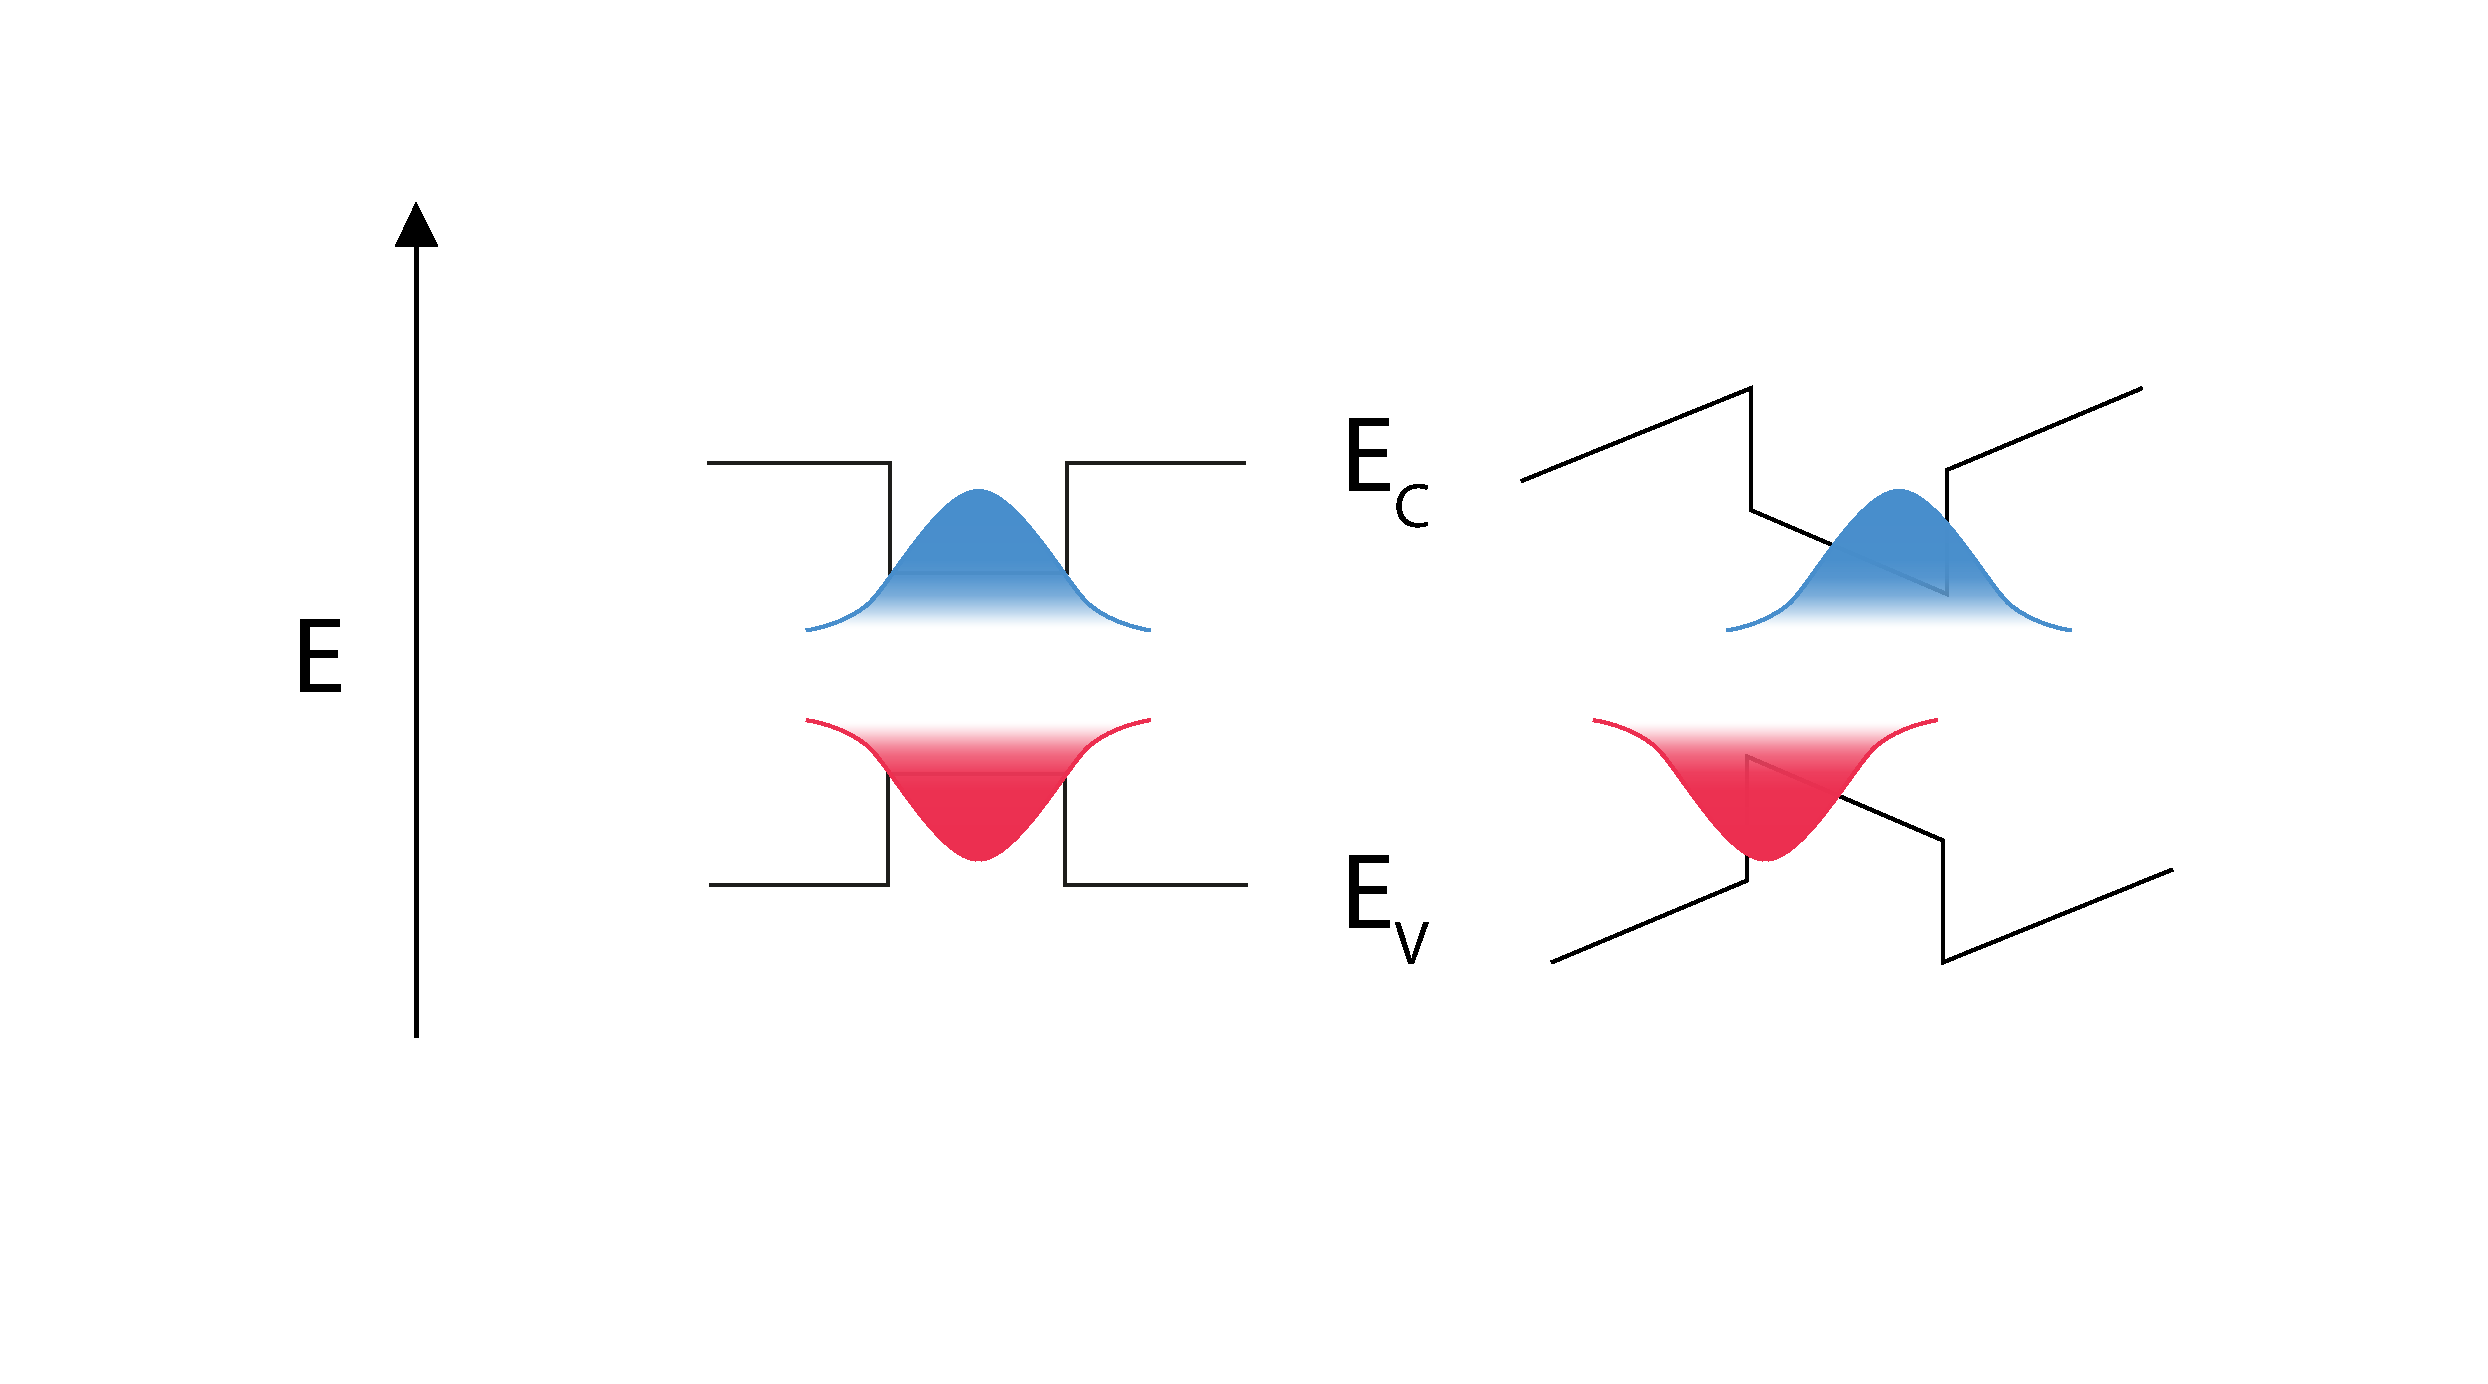
\includegraphics[width=\linewidth]{Bilder/QCSE.pdf}
        \caption{PL-Spektren der Proben ohne Übergitter}
    \end{minipage}% <- sonst wird hier ein Leerzeichen eingefügt
\end{figure}
\vspace{1cm}
\raggedright
\newpage
Die Ursache für die piezoelektrische Polarisation sind die Verspannungen zwischen den in (0001)-Richtung gewachsenen Schichten welche durch die unterschiedlichen thermischen Ausdehnungskoeffizienten und die Gitterfehlanpassung entstehen. Sie wird berechnet nach: 
%
\begin{equation}
    \vec{P}^{pz} = e \cdot \epsilon
\end{equation}
%
	
\chapter{Aufbau}


\thispagestyle{fancy}

\section{Photolumineszenzaufbau}

Für die experimentelle Untersuchung der UV-Photolumineszenz wurde der PL-Aufbau der AG-Kneissl verwendet, den Christoph Reich in der Zeit seiner Masterarbeit aufgebaut und während seiner Promotion erweitert hat~\cite{creich}. 
Als Anregungsquelle für die Photolumineszenz dient ein ArF-Excimerlaser mit einer Wellenlänge von $193 \ nm$ ($6,4 \ eV$). Mit dieser Wellenlänge ist er bestens geeignet für die Überbandanregung von Nitridhalbleitern. 
Des Weiteren bietet der Aufbau die Möglichkeit von temperaturabhängigen Untersuchungen von $5 \ K $ bis $300 K$. Dies ist auch die Grundlage für die Bestimmung der Internen Quanteneffizienz (kurz IQE), die den Großteil der Thematik dieser Arbeit ausmachen wird. 
\newline
Der Laser mit dem Modellnamen  "Xantos" von der Firma Coherent bietet eine maximale Emissionsenergie von $ 5 \ mJ $ und die Frequenz ist bis zu 500 Hz einstellbar bei einer Pulsdauer von $5 \ ns$. 
Durch interne Rückkopplung ist eine Energiestabilisierung möglich, die die Schwankung der Anregungsleistung auf 3 Prozent minimiert. 
\newline
Die Ansteuerung des kompletten Messvorgangs erfolgt durch die Messsoftware von Christoph Reich, entwickelt in der grafischen Programmiersprache "LabView" von Texas Instruments. Mit dieser ist es möglich alle nötigen Einstellungen an Pumpen, Heizern, Laser, Filtern und Spektrometer vorzunehmen, um einen komplett automatisierten Messvorgang zu starten, der nur noch aus Sicherheitsbedingungen überwacht werden muss. Spektren können so mit verschiedenen Parametern wie Position, Anregungsleistungsdichte, Temperatur, Energiebereich und Integrationszeit aufgenommen werden und auch ein Gaswechsel ist möglich.
\newline
Beginnend vom Laser wird im ersten Schritt der Lasterstrahl durch ein Linsensystem bestehend aus einer Zerstreuungs- und Sammellinse aufgeweitet. Dieser Schritt ermöglicht es, die Anregungsleistungsdichte zu verringern, um die am Aufbau beteiligten Gerätschaften nicht mit zu hohen Leistungen zu beschädigen. Damit sind insbesondere die Filterräder gemeint. Mit Hilfe der Filterräder ist es möglich, die Anregungsleistungsdichte 61 stufig zu variieren und somit leistungsdichteabhängige IQE Messungen zu machen. Als nächstes passiert der Strahl ein Linsensystem aus zwei Sammellinsen für eine Strahlverkleinerung. Vor dem Auftreffen des Strahles am Probenhalter im Kryostaten passiert der Strahl noch eine Lochblende. Sie dient der Entfernung achsennaher Strahlen und um bei Bedarf den Strahldruchmesser noch weiter zu verringern. Um den Strahl in Richtung des Probenhalters durch das Fenster im Kryostaten zu lenken, wird ein Spiegel mit einer dielektrischen Beschichtung benutzt. Der Laserstrahl durchdringt die Fenster des Kryostaten, diese sind speziell für eine hohe Transmission in diesem Wellenlängenbereich ausgelegt. Der Kryostat selbst ist horizontal und vertikal verfahrbar um die Messung mehrerer Proben im Probenhalter in einem Vorgang zu ermöglichen. Die Proben werden mit einem Kleber auf dem Probenhalter selbst befestigt, bevor dieser in den Kryostaten geschoben wird. 
Die Anregung der Proben mit dem Laserstrahl führt zur Proben spezifischen Emission von Licht. Diese wird von einer Linse im Strahlengang vor dem Detektor eingefangen und von einer zweiten Linse eingefangen die auf den Monochromatorspalt fokussiert ist.


	
\thispagestyle{fancy}

\section{Bestimmung der Degradation des UV Quarzglases}
%
\begin{figure}[htb]
  \centering
  \begin{minipage}[t]{0.49\linewidth}
      \centering
      \includegraphics[width=\linewidth]{Bilder/uvsilicaDegradation.png}
      \caption{Vom Hersteller angegebene wellenlängenabhängige Transmission vor und nach Degradation durch Bestrahlung.}
      \label{fig:degra}
  \end{minipage}
\end{figure}
\noindent
Da die Messung der Anregungsleistungdichte erfolgt, bevor das Laserlicht die Probe durch das UV-Quarzglas im Kryostaten trifft, ist es wichtig den Transmissionsverlust zu bestimmen, um die realen Werte für die Anregungsleistungsdichte zu kennen (Die Anregungsleistungsdichte, die bei der Probe ankommt). Der Kryostat besitzt vier Fenster, bestehend aus UV-Quarzglas, das besonders transparent im UV-Wellenlängenbereich ist. Durch diese Fenster dringt das Laserlicht in den Probenhalter ein. Von diesen Fenstern war und ist eines in dauerhaftem Gebrauch. Wie in Abbildung \ref{fig:degra} zu sehen ist, weisen die Fenster aber mit der fortlaufender Bestrahlung Degradation auf. So nimmt laut Hersteller durch Degradation die Transmission von 90 Prozent bis auf ca. 75 Prozent für eine Wellenlänge von 193 nm ab.
\newline
Um nun den Transmissongrad zu bestimmen, wurde der Probenhalter aus dem Kryostat entfernt, damit das Laserlicht ungehindert durch zwei parallel liegende Fenster durchdringen kann, um so auch die Anregungsleistungsdichte des Laserlichtes nach durchdringen des letzten Fenster messen zu können. So konnte die Anregungsleistungsdichte vor dem Eintreten und nach dem Austreten in den Kryostaten bestimmt werden. 
\newline
Dies wurde einmal bei den parallel liegenden unbenutzten Fenstern durchgeführt. Davon ausgehend, dass beide Fenster, da unbenutzt, den gleichen Transmissionsgrad haben, kann darauf zurückgeschlossen werden, dass ein unbenutztes Fenster einen Transmissionsgrad von 59 Prozent aufweist. Dies weicht um ca. 10 Prozent von der Herstellerangabe ab, die aber nicht die Reflektion im Kryostaten miteinbezieht. 
%
\begin{figure}[htb]
  \centering
  \begin{subfigure}{0.40\textwidth}
    \centering
    \includegraphics[width=0.9\linewidth]{Bilder/uvsilicavergleich.pdf}
    \caption{PL Intensität in Abhängigkeit der Anregungsleistungsdichte mit den benutzten und unbenutzten Fenstern}
    \label{fig:sub1}
  \end{subfigure}%
  {\LARGE$\xrightarrow{\cdot 0,44}$}
  \begin{subfigure}{0.40\textwidth}
    \centering
    \includegraphics[width=0.9\linewidth]{Bilder/uvsilicaVergleichSkaliert.pdf}
    \caption{Die Anregungsleistungsdichte des unbenutzten Fensters mit den rechnerisch bestimmten 0,44 skaliert}
    \label{fig:sub2}
  \end{subfigure}
  \caption{}
  \label{fig:vergleichSkaliert}
\end{figure}
\newline
Um den Transmissionsgrad des benutzten Fensters zu bestimmen, wurde die Transmission durch das benutzte und dem parallel liegende unbenutzte Fenster gemessen. Mit dem Wissen, dass der Transmissionsgrad durch das unbenutzte Fenster bei 59 Prozent ($T_{unb} = 0,59$) liegt, kann die Transmission durch das benutzte Fenster auf 26 Prozent ($T_{ben} = 0,26$) berechnet werden. 
Davon ausgehend, dass die Transmission bei höheren Wellenlängen (Emission) gleich und bei beiden Fenstern ähnlich ist,
%
\begin{equation}
  F_{skal} = \frac{ T_{ben} }{ T_{unb} } = 0,44\label{eq11}
\end{equation}
%
kann der Skalierungsfaktor mit für die Anregungsleistungsdichte auf 0.44 bestimmt werden. Dies bedeutet, dass durch Degradation die Transmission auf 44 Prozent der ursprünglichen Transmission gesunken ist.
\newline
Dies bestätigt sich auch durch die Gegenüberstellung in  Abbildung \ref{fig:vergleichSkaliert}. Somit ist durch die zeitliche Degradation die Transmission auf 44 Prozent der ursprünglichen gesunken. Dies bestätigt im Umkehrschluss, dass von der ausgehenden Anregungsleistungsdichte, die vor dem Kryostaten gemessen wird, durch die geringe Transmission der Fenster und Reflektion im und außerhalb des Kryostaten nur ca. 26 Prozent des vom Laser emittierten Lichtes bei der Probe ankommen. 

	\chapter{Ergebnisse}
\thispagestyle{fancy}
\section{Untersuchung optisch gepumpter Laserstrukturen auf unterschiedlichen Templates}


Dieses Kapitel widmet sich der Untersuchung der beiden Probenreihen TS4045 und TS4048 von optisch gepumpten Laserstrukturen die aus Rezepten aus zwei unterschiedlichen Serien stammen. Die beiden Serien unterscheiden sich im wesentlichen dadurch, dass sie mit(TS4048) und ohne Übergitter(TS4045) gewachsen wurden. Jede Reihe für sich weist  zusätzlich noch Unterschiede den Proben selbst auf, so sind zwei Proben der Reihe TS4045 auf AlN-Bulk zweier unterschiedlicher Hersteller (HexaTech, IKZ) gewachsen und alle  anderen Proben auf ELO AlN/Sapphire mit jeweils 3 unterschiedlichen "offcut"-Winkeln. Tabellerisch sieht die  Zusammenstellung wie folgt aus: 

\vspace{1cm}


\setlength{\arrayrulewidth}{0.5mm}
\setlength{\tabcolsep}{0.5pt}
\renewcommand{\arraystretch}{1.5}
 
{\rowcolors{3}{blue!80!yellow!50}{blue!70!yellow!40}
\begin{tabular}{ |p{2cm}|p{2cm}|p{2cm}|p{2cm}|p{2cm}|p{2cm}|   }
\hline
\multicolumn{3}{|c|}{TS4045} & \multicolumn{3}{c|}{TS4048}  \\
\hline
Endung & offcut& Template & Endung & offcut& Template \\
-2V* & 0.1$^\circ$m & ELO & -2V* & 0.1$^\circ$m & ELO \\
-2H & 0.1$^\circ$m & ELO & -2H & 0.1$^\circ$m & ELO \\
-2Z & 0.2$^\circ$m & ELO & -1 & 0.1$^\circ$m & ELO \\
-1 & 0.1$^\circ$m & Bulk (IKZ) & -2V* & 0.1$^\circ$m & ELO \\
-3* & 0.1$^\circ$m & Bulk (Hexatech) & -2V* & 0.1$^\circ$m & ELO \\



\end{tabular}
}



	\bibliography{Bibliographie}
\end{document}	


\begin{comment}
	\begin{figure}[b!]
    		\includegraphics[width=0.2\textwidth]{Bilder/TU-Berlin-Logo.pdf}
    		\label{fig:tulogo}
    	\end{figure}	
\end{comment}	
